%%%%%%%%%%%%%%%%%%%%%%%%%%%%%%%%%%%%
% Slide options
%%%%%%%%%%%%%%%%%%%%%%%%%%%%%%%%%%%%

% Option 1: Slides with solutions

\documentclass[slidestop,compress,mathserif]{beamer}
\newcommand{\soln}[1]{\textit{#1}}
\newcommand{\solnGr}[1]{#1}

% Option 2: Handouts without solutions

%\documentclass[11pt,containsverbatim,handout]{beamer}
%\usepackage{pgfpages}
%\pgfpagesuselayout{4 on 1}[letterpaper,landscape,border shrink=5mm]
%\newcommand{\soln}[1]{ }
%\newcommand{\solnGr}{ }


%%%%%%%%%%%%%%%%%%%%%%%%%%%%%%%%%%%%
% Style
%%%%%%%%%%%%%%%%%%%%%%%%%%%%%%%%%%%%

\def\chpiv@path{../../Chp 4}
\def\weekv@path{../../Week5}
\input{../../lec_style.tex}

%%%%%%%%%%%%%%%%%%%%%%%%%%%%%%%%%%%%
% Preamble
%%%%%%%%%%%%%%%%%%%%%%%%%%%%%%%%%%%%

\title[Lecture 14]{MA213: Lecture 14}
\subtitle{Module 2: Probability, Random Variables, and Distributions}
\author{OpenIntro Statistics, 4th Edition}
\institute{$\:$ \\ {\footnotesize Based on slides developed by Mine \c{C}etinkaya-Rundel of OpenIntro. \\
The slides may be copied, edited, and/or shared via the \webLink{http://creativecommons.org/licenses/by-sa/3.0/us/}{CC BY-SA license.} \\
Some images may be included under fair use guidelines (educational purposes).}}
\date{}

%%%%%%%%%%%%%%%%%%%%%%%%%%%%%%%%%%%%
% Begin document
%%%%%%%%%%%%%%%%%%%%%%%%%%%%%%%%%%%%

\begin{document}

%%%%%%%%%%%%%%%%%%%%%%%%%%%%%%%%%%%%
% Title page
%%%%%%%%%%%%%%%%%%%%%%%%%%%%%%%%%%%%

{
\addtocounter{framenumber}{-1} 
{\removepagenumbers 
\usebackgroundtemplate{\includegraphics[width=\paperwidth]{../../OpenIntro_Grid_4_3-01.jpg}}
\begin{frame}

\hfill \includegraphics[width=20mm]{../../oiLogo_highres}

\titlepage

\end{frame}
}
}


%%%%%%%%%%%%%%%%%%%%%%%%%%%%%%%%%%%%
% Recap/Agenda 
%%%%%%%%%%%%%%%%%%%%%%%%%%%%%%%%%%%%
% TODO better formatting
\begin{frame}
    \frametitle{Module 2: Probability, Random Variables, and Distributions}
    \begin{itemize}
        \item \hl{Previously: } Binomial distribution (Chapter 4.3)
        \item \hl{This time: } Poisson distribution (Chapter 4.5)
        \item \hl{Reading: } Chapter 5.1 for next time
        \item \hl{Deadlines/Announcements: } HW 5 due Monday
    \end{itemize}
    
\end{frame}
   
%%%%%%%%%%%%%%%%%%%%%%%%%%%%%%%%%%%%
% Learning objectives:
%%%%%%%%%%%%%%%%%%%%%%%%%%%%%%%%%%%%
\begin{frame}
    \frametitle{Learning Objectives}
    \begin{itemize}
        \item \textbf{M2 LO1: Validate and Explain Probability Distributions:} Assess the validity of a probability distribution using the concepts of outcome, sample space, and probability properties (e.g., disjoint outcomes, probabilities between 0 and 1, and total probabilities summing to 1).
        \item \textbf{M2 LO4: Understand and Compute Expectations and Variances:} Explain the concepts of expectations and variances of random variables, and compute the expectation and variance of a linear combination of random variables.
        %\item \textbf{M2 LO5: Model Data Using Bernoulli, Geometric, and Binomial Distributions:} Recognize when to appropriately model data using the Bernoulli, geometric, and binomial distributions, and compute quantities of interest such as mean, standard deviation, and tail probabilities.
        \item \textbf{M2 LO6: Assess Data Using the Normal Distribution:} Use the normal distribution to assess the "unusualness" of data points, apply the 68-95-99.7% rule, evaluate normality through histograms and q-q plots, and determine when a normal approximation to the binomial model is valid for calculating binomial probabilities.
    \end{itemize}
\end{frame}


%%%%%%%%%%%%%%%%%%%%%%%%%%%%%%%%%%%%
% Sections
%%%%%%%%%%%%%%%%%%%%%%%%%%%%%%%%%%%%

\begin{frame}
\frametitle{Binomial distribution}

\hl{Binomial distribution} describes the number of successes in a fixed number of \hl{iid} Bernoulli trials.

\begin{small}
$X \sim \text{Binomial}(n, p) \quad
Pr(X=k) = {n \choose k} p^k (1-p)^{n-k}, 
\quad k = 0, 1, 2, \ldots, n$
\end{small}
\vspace{-0.5cm}
\twocol{0.4}{0.6}{
    \begin{center}
        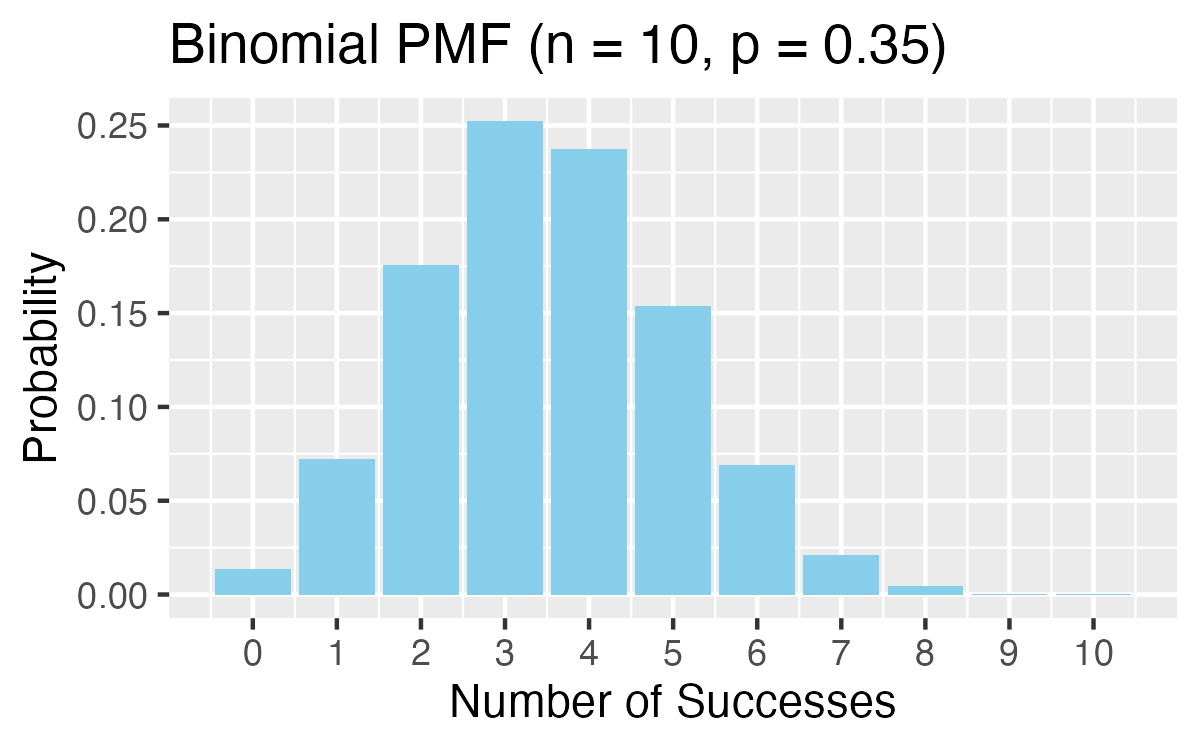
\includegraphics[width=0.35\paperwidth]{\weekv@path/figures/Binomial_PMF.png}
        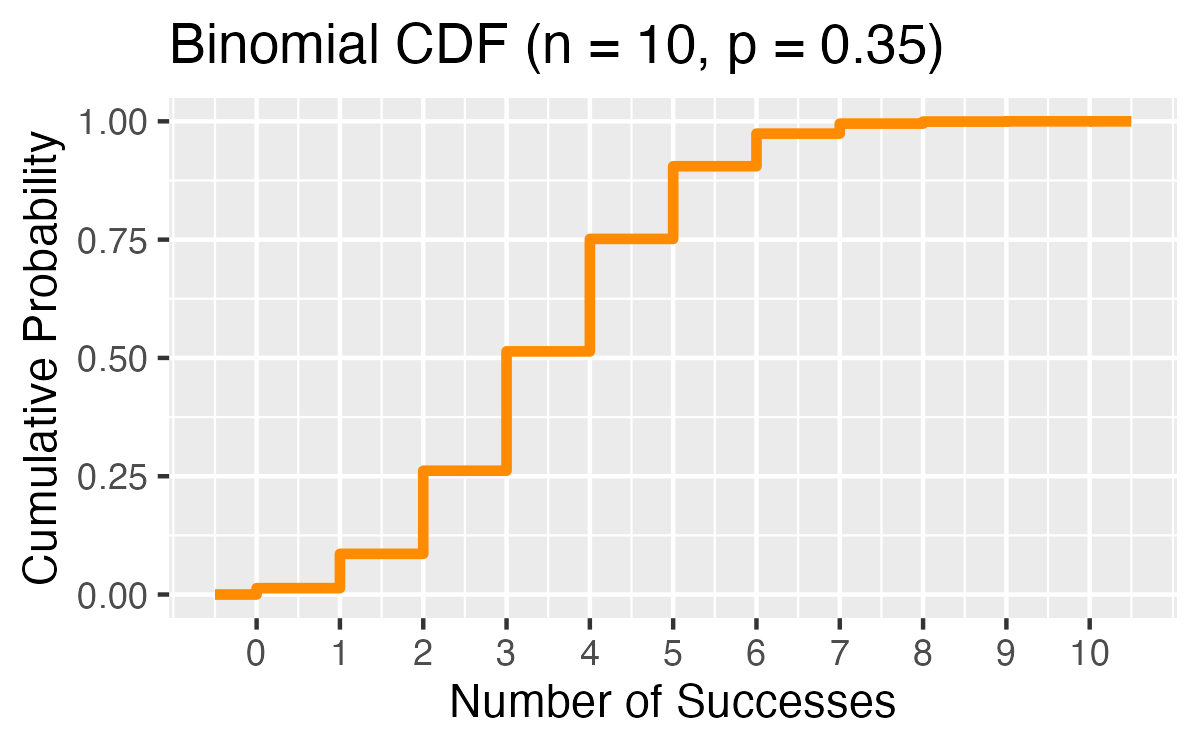
\includegraphics[width=0.35\paperwidth]{\weekv@path/figures/Binomial_CDF.png}
    \end{center}
}{
    % Binomial Distribution PMF Table
    \begin{small}
    \begin{center}
    \renewcommand{\arraystretch}{1.5}
    \begin{tabular}{l | c | c }
    Event                  & $X$   & $P(X)$                        \\
    \hline
    $0$ successes          & $0$   & ${n \choose 0} p^0 (1-p)^n$   \\
    $1$ success            & $1$   & ${n \choose 1} p^1 (1-p)^{n-1}$ \\
    $\vdots$               & $\vdots$ & $\vdots$                   \\
    $k$ successes          & $k$   & ${n \choose k} p^k (1-p)^{n-k}$ \\
    $\vdots$               & $\vdots$ & $\vdots$                   \\
    $n$ successes          & $n$   & ${n \choose n} p^n (1-p)^0$   \\
    \hline
    Total                  &       & $1$                           \\
    \end{tabular}
    \end{center}
    \end{small}
}

\end{frame}

%%%%%%%%%%%%%%%%%%%%%%%%%%%%%%%%%%%

\begin{frame}
\frametitle{Expected value and its variability}

\formula{Mean and standard deviation of binomial distribution}
{\[ \mu = np \qquad \qquad \sigma = \sqrt{np(1-p)} \] }

\pause

\begin{itemize}

\item Going back to the obesity rate:

\[ \sigma = \sqrt{np(1-p)} = \sqrt{100 \times 0.262 \times 0.738} \approx  4.4\]

\pause

\item We would expect 26.2 out of 100 randomly sampled Americans to be obese, with a standard deviation of 4.4.

\end{itemize}

\Note{Mean and standard deviation of a binomial might not always be whole numbers, and that is alright, these values represent what we would expect to see on average.}

\end{frame}

%%%%%%%%%%%%%%%%%%%%%%%%%%%%%%%%%%%

\begin{frame}
\frametitle{Unusual observations}

Using the notion that \hl{observations that are more than 2 standard deviations away from the mean are considered unusual} and the mean and the standard deviation we just computed, we can calculate a range for the plausible number of obese Americans in random samples of 100.

\[ 26.2 \pm (2 \times 4.4) = (17.4, 35) \]

\end{frame}

%%%%%%%%%%%%%%%%%%%%%%%%%%%%%%%%%%%%

\subsection{Normal approximation to the binomial}

%%%%%%%%%%%%%%%%%%%%%%%%%%%%%%%%%%%%

\section{R Demonstration: Sampling from the Binomial, Normal Approximation}
% Note: replacing slide below

%%%%%%%%%%%%%%%%%%%%%%%%%%%%%%%%%%%%

% \begin{frame}
% \frametitle{}

% \app{Shapes of binomial distributions}
% {
% For this activity you will use a web applet. Go to \webURL{https://gallery.shinyapps.io/dist_calc/} and choose Binomial coin experiment in the drop down menu on the left.
% \begin{itemize}
% \item Set the number of trials to 20 and the probability of success to 0.15. Describe the shape of the distribution of number of successes. 
% \item Keeping $p$ constant at 0.15, determine the minimum sample size required to obtain a unimodal and symmetric distribution of number of successes. Please submit only one response per team.
% \item Further considerations:
% \begin{itemize}
% \item What happens to the shape of the distribution as $n$ stays constant and $p$ changes?
% \item What happens to the shape of the distribution as $p$ stays constant and $n$ changes?
% \end{itemize}
% \end{itemize}
% }

% \end{frame}

%%%%%%%%%%%%%%%%%%%%%%%%%%%%%%%%%%%%

\begin{frame}
\frametitle{Distributions of number of successes}

\dq{Hollow histograms of samples from the binomial model where $p = 0.10$ and $n = 10$, $30$, $100$, and $300$. What happens as $n$ increases?}

\begin{center}
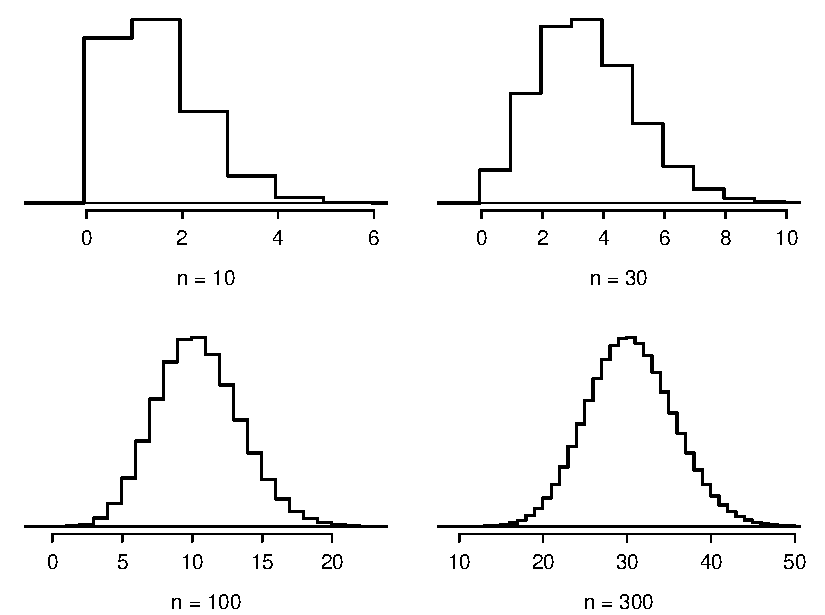
\includegraphics[width=0.60\textwidth]{\chpiv@path/4-3_binomial_distribution/figures/fourBinomialModelsShowingApproxToNormal/fourBinomialModelsShowingApproxToNormal}
\end{center}

\end{frame}

%%%%%%%%%%%%%%%%%%%%%%%%%%%%%%%%%%%

\begin{frame}
\frametitle{How large is large enough?}

The sample size is considered large enough to use a Normal approximation if the expected number of successes and failures are both at least 10.
\[ np \ge 10 \qquad \text{ and } \qquad n(1-p) \ge 10 \]

\soln{\only<2->{$10 \times 0.13 = 1.3; 10 \times (1 - 0.13) = 8.7$}}

\end{frame}

%%%%%%%%%%%%%%%%%%%%%%%%%%%%%%%%%%

\begin{frame}
\frametitle{}

\pq{Below are four pairs of Binomial distribution parameters. Which distribution can be approximated by the normal distribution?}

\begin{enumerate}[(a)]
\item $n = 100, p = 0.95$
\solnMult{$n = 25, p = 0.45$} \soln{\only<2>{\orange{$\rightarrow 25 \times 0.45 = 11.25; 25 \times 0.55 = 13.75$}}}
\item $n = 150, p = 0.05$
\item $n = 500, p = 0.015$
\end{enumerate}

\end{frame}


%%%%%%%%%%%%%%%%%%%%%%%%%%%%%%%%%%%%

\section{Edfinity quiz: Modeling with the Binomial distribution}

%%%%%%%%%%%%%%%%%%%%%%%%%%%%%%%%%%%%


% \begin{frame}
% \frametitle{An analysis of Facebook users}

% \dq{A study found that ``Facebook users get more than they give". For example:
% \begin{itemize}
% \item 40\% of Facebook users in our sample made a friend request, but 63\% received at least one request
% \item Users in our sample pressed the like button next to friends' content an average of 14 times, but had their content ``liked" an average of 20 times
% \item Users sent 9 personal messages, but received 12
% \item 12\% of users tagged a friend in a photo, but 35\% were themselves tagged in a photo
% \end{itemize}
% Any guesses for how this pattern can be explained?
% }

% \soln{\only<2>{Power users contribute much more content than the typical user.}}

% \ct{\webURL{http://www.pewinternet.org/Reports/2012/Facebook-users/Summary.aspx}}

% \end{frame}

%%%%%%%%%%%%%%%%%%%%%%%%%%%%%%%%%%%

\begin{frame}
\frametitle{}

\dq{A 2012 study found that found that approximately 25\% of Facebook users are considered power users. The same study found that the average Facebook user has 245 friends. What is the probability that the average Facebook user with 245 friends has 70 or more friends who would be considered power users? Note any assumptions you must make.}

We are given that $n = 245, p = 0.25$, and we are asked for the probability $P(X \ge 70)$. To proceed, we need independence, which we'll assume. So then $X\sim Binomial(245,0.25)$.

\pause

\begin{align*}
P(X \ge 70) &= P(X = 70\text{ or }X = 71\text{ or }X = 72\text{ or }\cdots\text{ or } X = 245) \\
&= P(X = 70) + P(X = 71) + P(X = 72) + \cdots + P(X = 245)
\end{align*}

\pause

This seems like an awful lot of work...

\end{frame}

%%%%%%%%%%%%%%%%%%%%%%%%%%%%%%%%%%%

\begin{frame}
\frametitle{Normal approximation to the binomial}

When the sample size is large enough, the binomial distribution with parameters $n$ and $p$ can be approximated by the normal model with parameters $\mu = np$ and $\sigma = \sqrt{np(1-p)}$.

\begin{itemize}

\item In the case of the Facebook power users, $n = 245$ and $p = 0.25$.
\[ \mu = 245 \times 0.25 = 61.25 \qquad \sigma = \sqrt{245 \times 0.25 \times 0.75} = 6.78 \]

\item $Bin(n = 245, p = 0.25) \approx N(\mu = 61.25, \sigma = 6.78)$.

\begin{center}
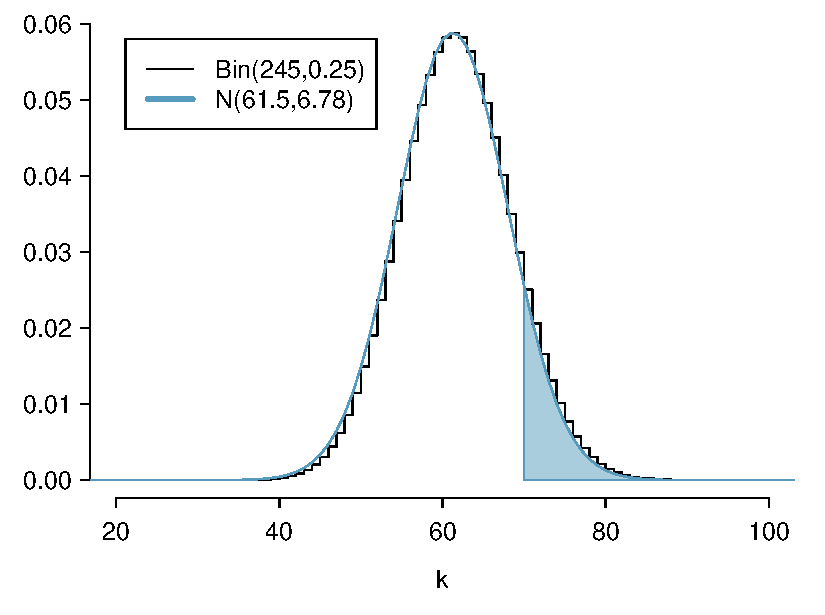
\includegraphics[width=0.5\textwidth]{\chpiv@path/4-3_binomial_distribution/figures/fb_power_user/fb_power_user}
\end{center}

\end{itemize}

\end{frame}

%%%%%%%%%%%%%%%%%%%%%%%%%%%%%%%%%

\begin{frame}[fragile]
\frametitle{}

\dq{What is the probability that the average Facebook user with 245 friends has 70 or more friends who would be considered power users?}

\twocol{0.5}{0.5}{
\begin{center}
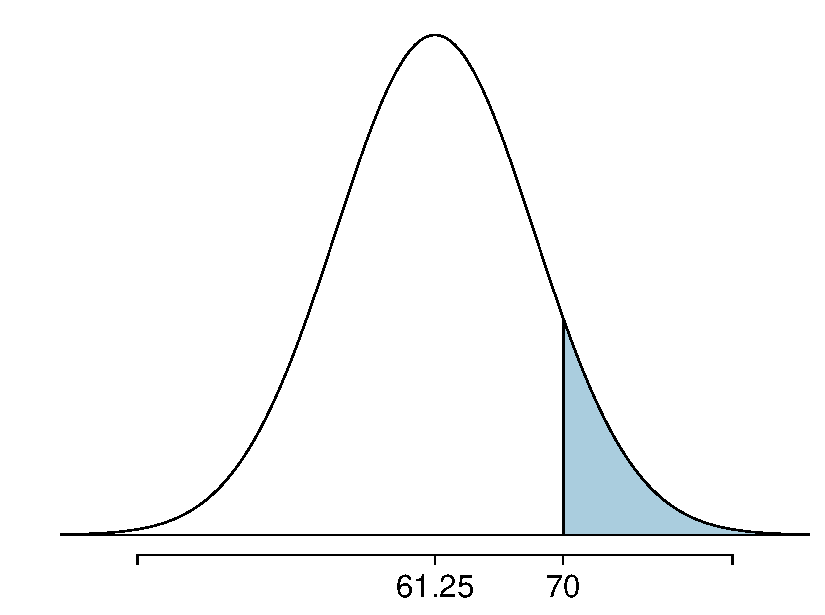
\includegraphics[width=\textwidth]{\chpiv@path/4-3_binomial_distribution/figures/fb_power_user/fb_power_user_norm}
\end{center}
}
{
\[ Z = \frac{obs - mean}{SD} = \frac{70 - 61.25}{6.78} = 1.29 \]
\[ P(Z > 1.29) = 1 - 0.9015 = 0.0985 \]
}

\begin{beamerboxesrounded}[shadow = true, lower = code body]{}
{\small \begin{verbatim}
> 1 - pnorm(1.29)
[1] 0.09852533
> 1 - pnorm(70, mean = 61.25, sd = 6.78)
[1] 0.09842807
\end{verbatim}
}
\end{beamerboxesrounded}

\end{frame}

%%%%%%%%%%%%%%%%%%%%%%%%%%%%%%%%%

\subsection{The normal approximation breaks down on small intervals}

%%%%%%%%%%%%%%%%%%%%%%%%%%%%%%%%%%%%

\begin{frame}
\frametitle{The normal approximation breaks down on small intervals}

\begin{itemize}

\item The normal approximation to the binomial distribution tends to perform poorly when estimating the probability of a small range of counts, even when the conditions are met.

\item This approximation for intervals of values is usually improved if cutoff values are extended by 0.5 in either direction, depending on the desired range.

\end{itemize}

\twocol{0.5}{0.5}{
\begin{small}
\begin{center}
For example:
\begin{itemize}
    \item For $Pr(B=a)$, compute $Pr(a-0.5<X<a+0.5)$
    \item For $Pr(B<a)$, compute $Pr(X<a-0.5)$
    \item For $Pr(B\le a)$, compute $Pr(X<a+0.5)$
\end{itemize}
\end{center}
\end{small}
}{
\begin{center}
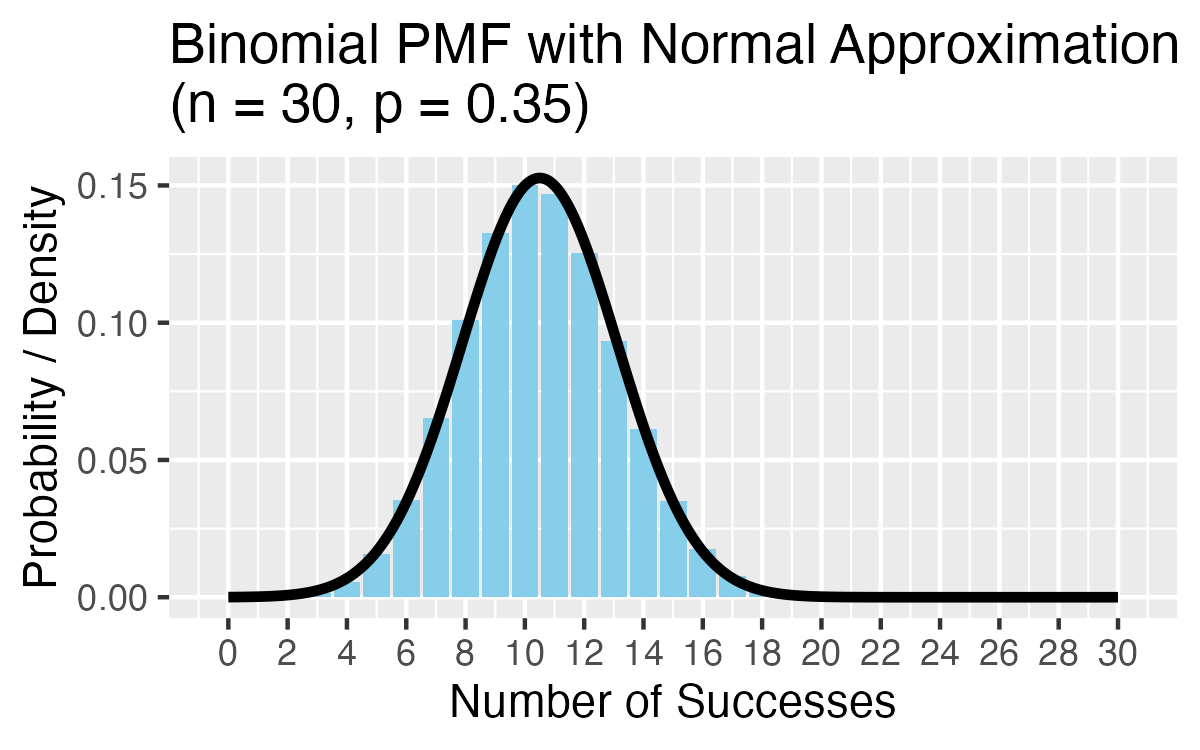
\includegraphics[width=0.45\paperwidth]{\weekv@path/figures/Binomial_PMF_Normal.png}
\end{center}
}

\end{frame}

%%%%%%%%%%%%%%%%%%%%%%%%%%%%%%%%%%

%%%%%%%%%%%%%%%%%%%%%%%%%%%%%%%%%%%%

\section{Poisson distribution}

%%%%%%%%%%%%%%%%%%%%%%%%%%%%%%%%%%%%

\begin{frame}
\frametitle{Poisson distribution}

\begin{itemize}

\item The \hl{Poisson distribution} is often useful for modeling the \hl{count} of events in a given interval of time (or space), when these events occur with a known rate and independently of the time since the last event.

\item The \hl{rate} for a Poisson distribution is the average number of occurrences per unit of time, and is typically denoted by \mathhl{\lambda}.

\item Using the rate, we can describe the probability of observing exactly $k$ events in a single unit of time.

\end{itemize}

\vfill

\formula{Poisson distribution}
{
\orange{P(observe $k$ events) = $\frac{\lambda^k e^{-\lambda}}{k!} \qquad k=0, 1, 2, 3, ...$}\\
The constant $e \approx 2.718$ is Euler's number. \\

\orange{$E[X]=\lambda \qquad Var(X)=\lambda \qquad SD(X)=\sqrt{\lambda}$}
}

\end{frame}

%%%%%%%%%%%%%%%%%%%%%%%%%%%%%%%%%%
\begin{frame}
\frametitle{Poisson distribution}

The \hl{Poisson distribution} models the count of events occurring in a fixed interval of time or space, given a constant average rate and independence between events.

\begin{small}
$X \sim \text{Poisson}(\lambda) \quad
Pr(X=k) = \frac{\lambda^k e^{-\lambda}}{k!}, 
\quad k = 0, 1, 2, \ldots$
\end{small}
% \vspace{-0.5cm}
\twocol{0.4}{0.6}{
    \begin{center}
        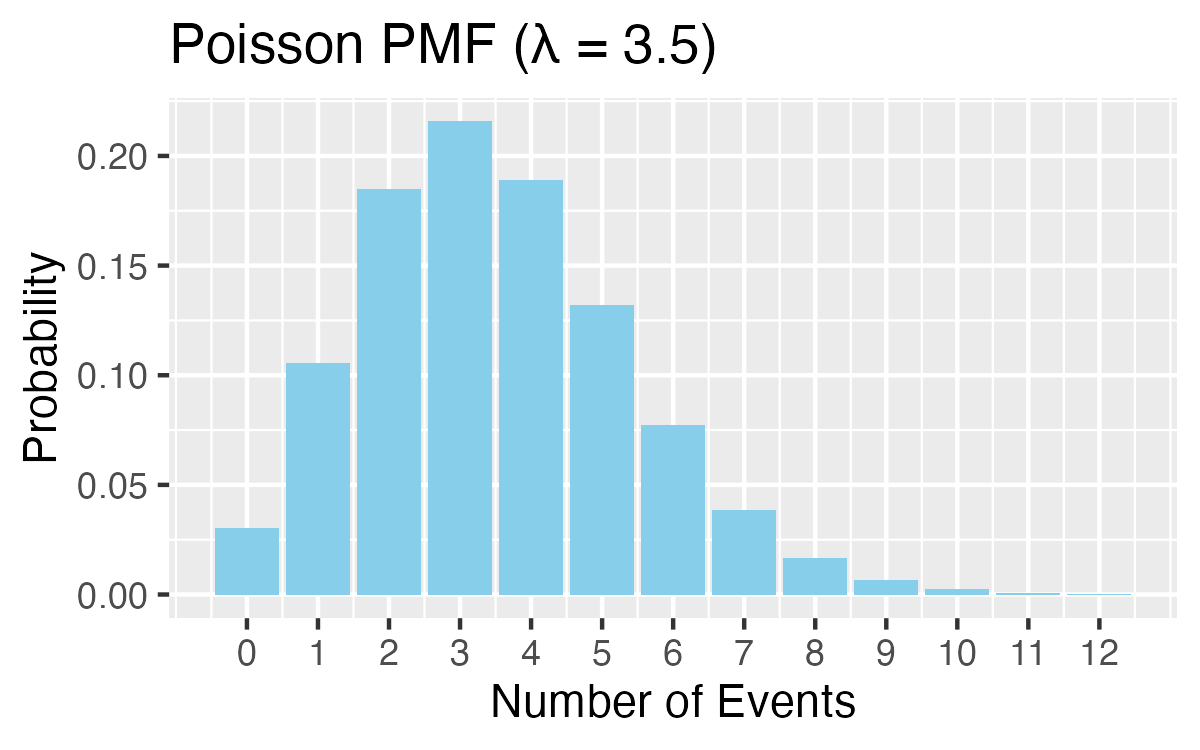
\includegraphics[height=0.25\paperheight]{\weekv@path/figures/Poisson_PMF.png}
        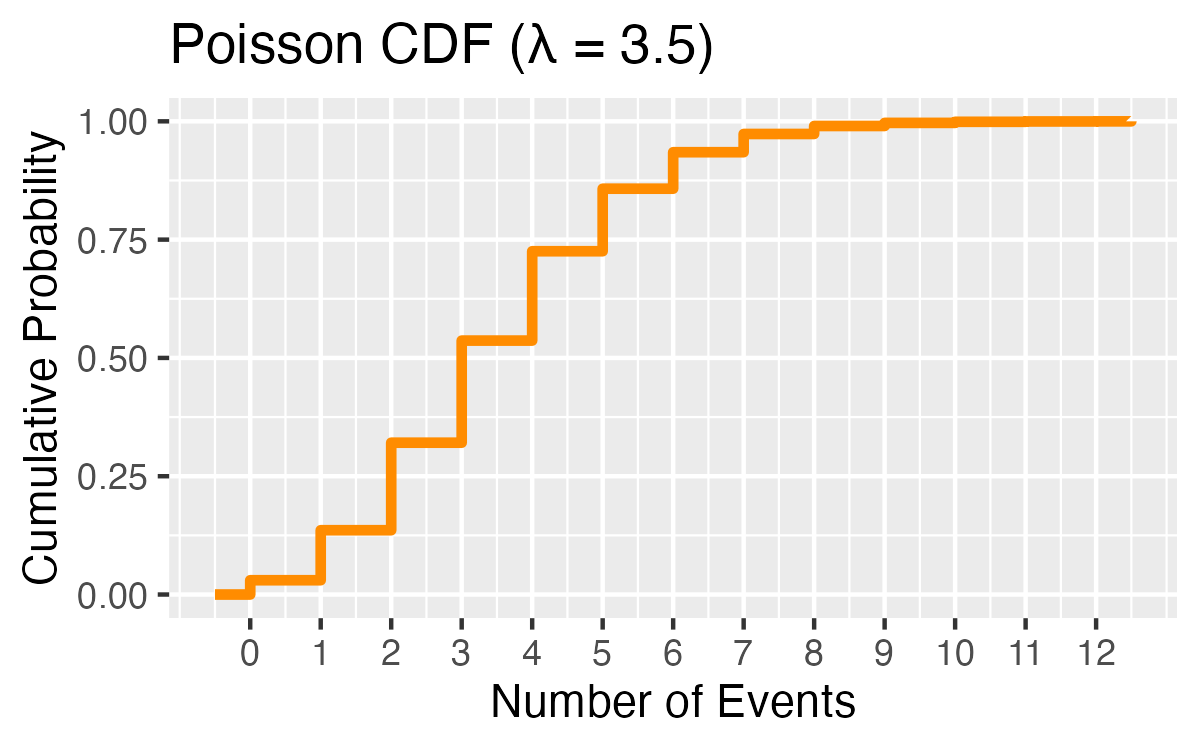
\includegraphics[height=0.25\paperheight]{\weekv@path/figures/Poisson_CDF.png}
    \end{center}
}{
    % Poisson Distribution PMF Table
    \begin{small}
    \begin{center}
    \renewcommand{\arraystretch}{1.5}
    \begin{tabular}{l | c | c }
    Event                  & $X$   & $P(X)$                        \\
    \hline
    $0$ events             & $0$   & $e^{-\lambda}$   \\
    $1$ event              & $1$   & $\frac{\lambda^1 e^{-\lambda}}{1!}$   \\
    $\vdots$               & $\vdots$ & $\vdots$                   \\
    $k$ events             & $k$   & $\frac{\lambda^k e^{-\lambda}}{k!}$   \\
    $\vdots$               & $\vdots$ & $\vdots$                   \\
    \hline
    Total                  &       & $1$                           \\
    \end{tabular}
    \end{center}
    \end{small}
}

\end{frame}
%%%%%%%%%%%%%%%%%%%%%%%%%%%%%%%%%%%%

\begin{frame}

\dq{Suppose that in a rural region of a developing country electricity power failures occur following a Poisson distribution with an average of 2 failures every week. Calculate the probability that in a given week the electricity fails only once.}

\pause

$X \sim Poisson(\lambda = 2)$

\pause

\begin{eqnarray*}
P(\text{only 1 failure in a week}) &=& Pr(X=1)\\
&=& \frac{2^1 \times e^{-2}}{1!} \\
\pause
&=& \frac{2 \times e^{-2}}{1} \\
\pause
&=& 0.27
\end{eqnarray*}

\end{frame}

%%%%%%%%%%%%%%%%%%%%%%%%%%%%%%%%%%%%

\begin{frame}

\dq{Suppose that in a rural region of a developing country electricity power failures occur following a Poisson distribution with an average of 2 failures every week. Calculate the probability that on a given \underline{day} the electricity fails three times.}

\pause

We are given the weekly failure rate, but to answer this question we need to first calculate the average rate of failure on a given day: $\lambda_{day} = \frac{2}{7} = 0.2857$. Note that we are assuming that the probability of power failure is the same on any day of the week, i.e. we assume independence.

\pause

\begin{eqnarray*}
P(\text{3 failures on a given day}) &=& \frac{0.2857^3 \times e^{-0.2857}}{3!} \\
\pause
&=& \frac{0.2857^3 \times e^{-0.2857}}{6} \\
\pause
&=& 0.0029
\end{eqnarray*}

\end{frame}

%%%%%%%%%%%%%%%%%%%%%%%%%%%%%%%%%%%%

\section{R Demonstration: Sampling from the Poisson distribution}

%%%%%%%%%%%%%%%%%%%%%%%%%%%%%%%%%%%%

\section{Edfinity quiz: Modeling with the Poisson distribution}

%%%%%%%%%%%%%%%%%%%%%%%%%%%%%%%%%%%%

\begin{frame}
\frametitle{Is it Poisson?}
\begin{small}
\begin{itemize}

\item A random variable may follow a Poisson distribution if the events occur independently of each other (typically, when the population is large and the events are rare) and the rate of events is constant

\item However we can think of situations where the rate is not constant. For example, if we are interested in count of weddings over one summer, we should take into consideration that weekends are more popular for weddings.

\item In this case, a Poisson model may sometimes still be reasonable if we allow it to have a different rate for different times; we could model the rate as higher on weekends than on weekdays.

\item The idea of modeling rates for a Poisson distribution against a second variable (day of the week) forms the
foundation of some more advanced methods called \hl{generalized linear models}. There are beyond the scope of this course, but we will discuss a foundation of linear models in Chapters 7 and 8.

\end{itemize}
\end{small}

\end{frame}

%%%%%%%%%%%%%%%%%%%%%%%%%%%%

\begin{frame}
\frametitle{Comparing Binomial and Poisson Distributions}

The Poisson and Binomial distributions both count occurrences of independent events

\vspace{0.3cm}

\begin{tabular}{|p{0.45\textwidth}|p{0.45\textwidth}|}
\hline
\rowcolor{gray!20}
\textbf{Binomial $(n, p)$} & \textbf{Poisson $(\lambda)$} \\
\hline
Counting \# successes out of $n$ trials, each with probability $p$ & Counting \# events in a time (or space) interval, with rate $\lambda$ \\
\hline
Trials are independent & Events are independent \\
\hline
$Pr(X = x) = \dbinom{n}{x} p^x (1-p)^{n-x}$ \newline $x \in \{0,1,2,\ldots,n\}$ & $Pr(X = x) = \dfrac{\lambda^x e^{-\lambda}}{x!}$ \newline $x \in \{0,1,2,\ldots\}$ \\
\hline
$E[X] = np$ & $E[X] = \lambda$ \\
\hline
$Var[X] = np(1-p)$ & $Var[X] = \lambda$ \\
\hline
\end{tabular}

\end{frame}

%%%%%%%%%%%%%%%%%%%%%%%%%%%%%%%%%%%%

\begin{frame}
\frametitle{How are the Poisson and Binomial distributions related?}

\begin{small}
Suppose that about 5 trains arrive at BU West per hour. $X$ is the number of trains that arrive 9am--10am.
    \begin{itemize}
        \item $X \sim \text{Poisson}(5)$, where rate $\lambda = 5$ trains/hour
    \end{itemize}
    \pause
Approximately, we can split the hour into 10 intervals, each 6 minutes long:
    \begin{itemize}
        \item $Pr(\text{train in each subinterval}) = p = \lambda/10 = 0.5$
        \item 10 trials, each with probability 0.5 of success
        \item $\text{Poisson}(5) \approx \text{Binomial}(10, 0.5)$
        \item \textcolor{teal}{\fbox{Has the same expected number of trains: $np = \lambda = 5$}}
        \item \textcolor{teal}{\fbox{Doesn't account for if 2 trains arrive in one 6 minute interval}}
    \end{itemize}

\end{small}

\end{frame}

%%%%%%%%%%%%%%%%%%%%%%%%%%%%%%%%%%%%

\begin{frame}
\frametitle{How are the Poisson and Binomial distributions related?}

\begin{small}
Suppose that about 5 trains arrive at BU West per hour. $X$ is the number of trains that arrive 9am--10am.
    \begin{itemize}
        \item $X \sim \text{Poisson}(5)$, where rate $\lambda = 5$ trains/hour
    \end{itemize}
    
Or, split the hour into 100 subintervals, each 0.6 minutes long:
    \begin{itemize}
        \item $Pr(\text{train in each subinterval}) = p = \lambda/100 = 0.05$
        \item 100 trials, each with probability 0.05 of success
        \item $\text{Poisson}(5) \approx \text{Binomial}(100, 0.05)$
        \item \textcolor{teal}{\fbox{Has the same expected number of trains: $np = \lambda = 5$}}
        \item \textcolor{teal}{\fbox{Doesn't account for if 2 trains arrive in one 0.6 minute interval}}
    \end{itemize}
    \pause
The approximation gets better as we increase the number of subintervals $n$ (``large population"), while reducing $p$ at the same time (``rare events") so that $np = \lambda$ is kept constant.

\end{small}

\end{frame}

%%%%%%%%%%%%%%%%%%%%%%%%%%%%%%%%%%%%

\section{R Demonstration: Relationship between Poisson and Binomial}

%%%%%%%%%%%%%%%%%%%%%%%%%%%%%%%%%%%%

% \begin{frame}
% \frametitle{Practice}

% \pq{A random variable that follows which of the following distributions can take on values other than positive integers?}

% \begin{enumerate}[(a)]
% \item Poisson
% \item Negative binomial
% \item Binomial
% \solnMult{Normal}
% \item Geometric
% \end{enumerate}

% \end{frame}


%%%%%%%%%%%%%%%%%%%%%%%%%%%%%%%%%%%%
% End document
%%%%%%%%%%%%%%%%%%%%%%%%%%%%%%%%%%%%

\end{document}